% shared-layout-id: 86b69ef0c611a25f6e0e456b91c2adc284c301dbe992a69289aec0fcd8e7dcc1
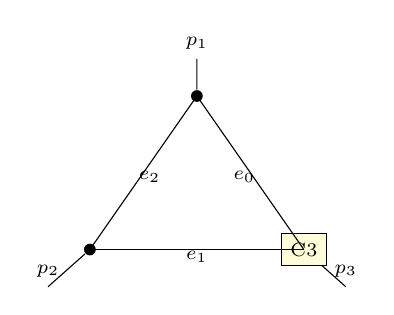
\begin{tikzpicture}[scale=.65,every node/.style={font=\scriptsize}]
\node[rectangle,draw,fill=yellow!15] (v0) at (5.36363636,1.18181818) {C3};
\node[circle,fill,inner sep=1.5pt] (v1) at (3.27272727,4.18181818) {};
\node[circle,fill,inner sep=1.5pt] (v2) at (1.18181818,1.18181818) {};
\draw[black] (5.36363636,1.18181818) .. controls (4.66666667,2.18181818) and (3.96969697,3.18181818) .. (3.27272727,4.18181818);
\node at (4.19885118,2.59864834) {$e_{0}$};
\draw[black] (5.36363636,1.18181818) .. controls (3.96969697,1.18181818) and (2.57575758,1.18181818) .. (1.18181818,1.18181818);
\node at (3.27272727,1.03636364) {$e_{1}$};
\draw[black] (3.27272727,4.18181818) .. controls (2.57575758,3.18181818) and (1.87878788,2.18181818) .. (1.18181818,1.18181818);
\node at (2.34660337,2.59864834) {$e_{2}$};
\draw (v1) -- (3.27272727,4.90909091) node[above] {$p_{1}$};
\draw (v2) -- (0.36363636,0.45454545) node[above] {$p_{2}$};
\draw (v0) -- (6.18181818,0.45454545) node[above] {$p_{3}$};
\end{tikzpicture}